
\subsection{Technische Erkenntnisse}

\textbf{Problemlösung durch Constraints:}

\raggedright Die Infrarot-Pipeline entwickelte sich aus spezifischen Produktionsanforderungen und praktischen Constraints. MediaPipes Verarbeitungsfähigkeit für Infrarot-Daten wurde empirisch validiert und für die Projektanforderungen angepasst. Diese Erfahrung verdeutlichte, wie praxisorientierte Lösungsansätze zur Systemoptimierung beitragen können.

\textbf{Architektonische Evolution:}

\raggedright Der Projektverlauf dokumentiert eine schrittweise Vereinfachung: Von der geplanten Dual-Sensor-Fusion mit Kalman-Filter zu einer reinen MediaPipe-Lösung. Jede Reduktion verbesserte Stabilität und Wartbarkeit. Die finale Architektur ist nicht die technisch komplexeste, aber die praktikabelste.

\textbf{Modularität als Designprinzip:}

\raggedright Die Entscheidung, jeden Aspekt (Tracking, Analyse, Visualisierung) in separate TouchDesigner-Container zu kapseln, erwies sich als fundamental. Sie ermöglichte nicht nur parallele Entwicklung, sondern macht das System zukunftssicher: Neue Tracking-Technologien können ohne Änderung der Visualisierungslogik integriert werden.

\textbf{Projektmanagement im interdisziplinären Kontext:}

\textbf{Adaptive Planung:}

\raggedright Die Sprint-Struktur musste mehrfach angepasst werden. Choreographische Anforderungen entstanden organisch während der Proben, nicht durch Requirements Engineering. Sprint 3 wurde komplett umgeplant, als die handgezeichneten Visual-Konzepte eintrafen. Diese Flexibilität war keine Schwäche, sondern Stärke des Prozesses.

\textbf{Dokumentation als Kommunikationswerkzeug:}

\raggedright Die parallele Dokumentation diente nicht nur der Nachvollziehbarkeit, sondern wurde zum primären Kommunikationsmedium mit den Stakeholdern. Screenshots und Diagramme überbrückten die Sprachbarriere zwischen Technik und Kunst effektiver als verbale Erklärungen.

\textbf{Solo-Development-Strategien:}

\raggedright Als Alleinentwickler musste ich spezifische Strategien für die Stakeholder-Kommunikation entwickeln:

\textbf{Erfolgreiche Ansätze:}
\begin{itemize}
\item \textbf{Regelmäßige Demo-Sessions:} Konkrete Fortschritte reduzierten Stakeholder-Unsicherheit
\item \textbf{Transparente Dokumentation:} GitHub-Repository und .toe-Dateien als Kommunikationsbasis
\item \textbf{Proaktive Problem-Kommunikation:} Frühe Information bei technischen Herausforderungen
\item \textbf{Sprint-synchronisierte Updates:} Strukturierte 2-3 Wochen Kommunikationsrhythmus
\end{itemize}

\textbf{Herausforderungen der Solo-Entwicklung:}
\begin{itemize}
\item \textbf{Isolation bei technischen Problemen:} Eigenständige Problemlösung zeitaufwändig
\item \textbf{Stakeholder-Erwartungsmanagement:} Balance zwischen Ambition und Realisierbarkeit
\item \textbf{Dokumentations-Overhead:} Umfassende Dokumentation für interdisziplinäre Kommunikation
\end{itemize}

\begin{figure}[htbp]
    \centering
    \adjustbox{max width=0.9\textwidth, max height=0.8\textheight, keepaspectratio}{%
        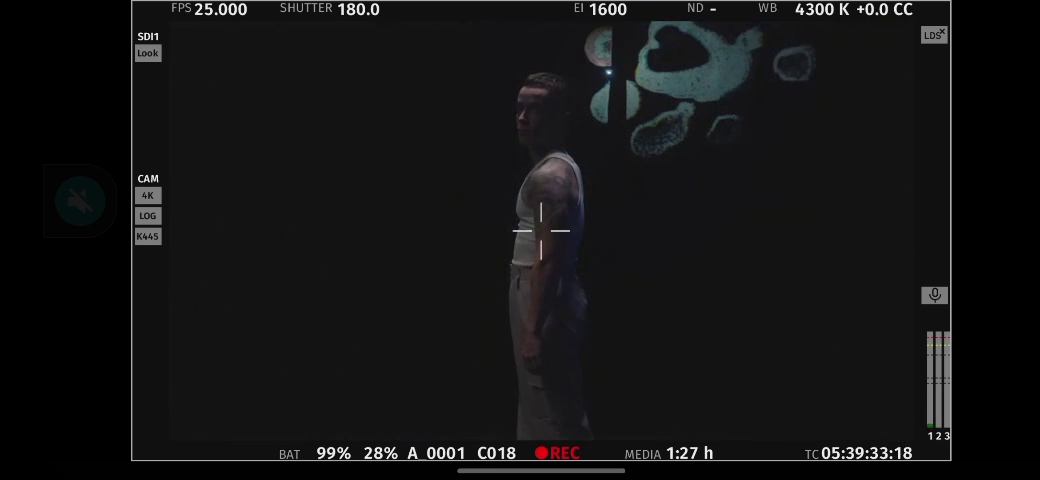
\includegraphics{images/onSetImages/HeadTracking_HQCamera.png}%
    }
    \caption{Kopfpartikel-Setup: Komplexe Kamera-Beamer-Ausrichtung mit hardcoded Offsets in particleGPU je nach Kamera-Winkel, was zu einer Erhöhung der Zeit zwischen Takes führte}
    \label{fig:head_setup}
\end{figure}

\textbf{Kollaboration über Disziplingrenzen:}

\textbf{Visuelle Kommunikation:}

\raggedright Die wichtigste Herausforderung war die Übersetzung zwischen künstlerischer Vision und technischer Implementation. „Es soll aussehen wie Gedanken, die explodieren" musste in Partikel-Emissionsraten und Geschwindigkeitsvektoren übersetzt werden. Die Lösung: Rapid Prototyping mit sofortigem visuellem Feedback.

\textbf{Gegenseitiges Lernen:}

\raggedright Das Filmteam lernte technische Constraints zu respektieren (MediaPipe braucht Kontrast), ich lernte künstlerische Prioritäten zu verstehen (Effekt vor Präzision). Diese gegenseitige Bildung war wertvoll über das Projekt hinaus.

\textbf{Iterative Stakeholder-Integration:}

Schlüsselmomente der Zusammenarbeit prägten die Entwicklungsrichtung:
\begin{itemize}
\item \textbf{Frühe Expertenberatung:} Technical Review (17.01.2025) definierte Projektrichtung
\item \textbf{Stakeholder-Integration:} Choreographie-Meeting (10.03.2025) prägte Entwicklung
\item \textbf{Iterative Validation:} Kontinuierliche Demo-Sessions verhinderten Fehlentwicklung
\item \textbf{Lösungen durch Notwendigkeit:} Produktionsanforderungen führten zu praktischen technischen Anpassungen
\end{itemize}

\textbf{Produktionsumgebung und Systemvalidierung:}

\textbf{Echtzeit-Anforderungen:}

\raggedright Die Produktionsumgebung erforderte robuste Systemarchitektur mit minimalen Ausfallzeiten. Entwickelte Debug-Visualisierungen dienten gleichzeitig als Produktionsmonitoring-Tools. Die Echtzeit-Skelett-Overlays erwiesen sich als essentiell für die operative Systemüberwachung während der Aufnahmen.

\begin{figure}[htbp]
    \centering
    \adjustbox{max width=0.8\textwidth, max height=0.8\textheight, keepaspectratio}{%
        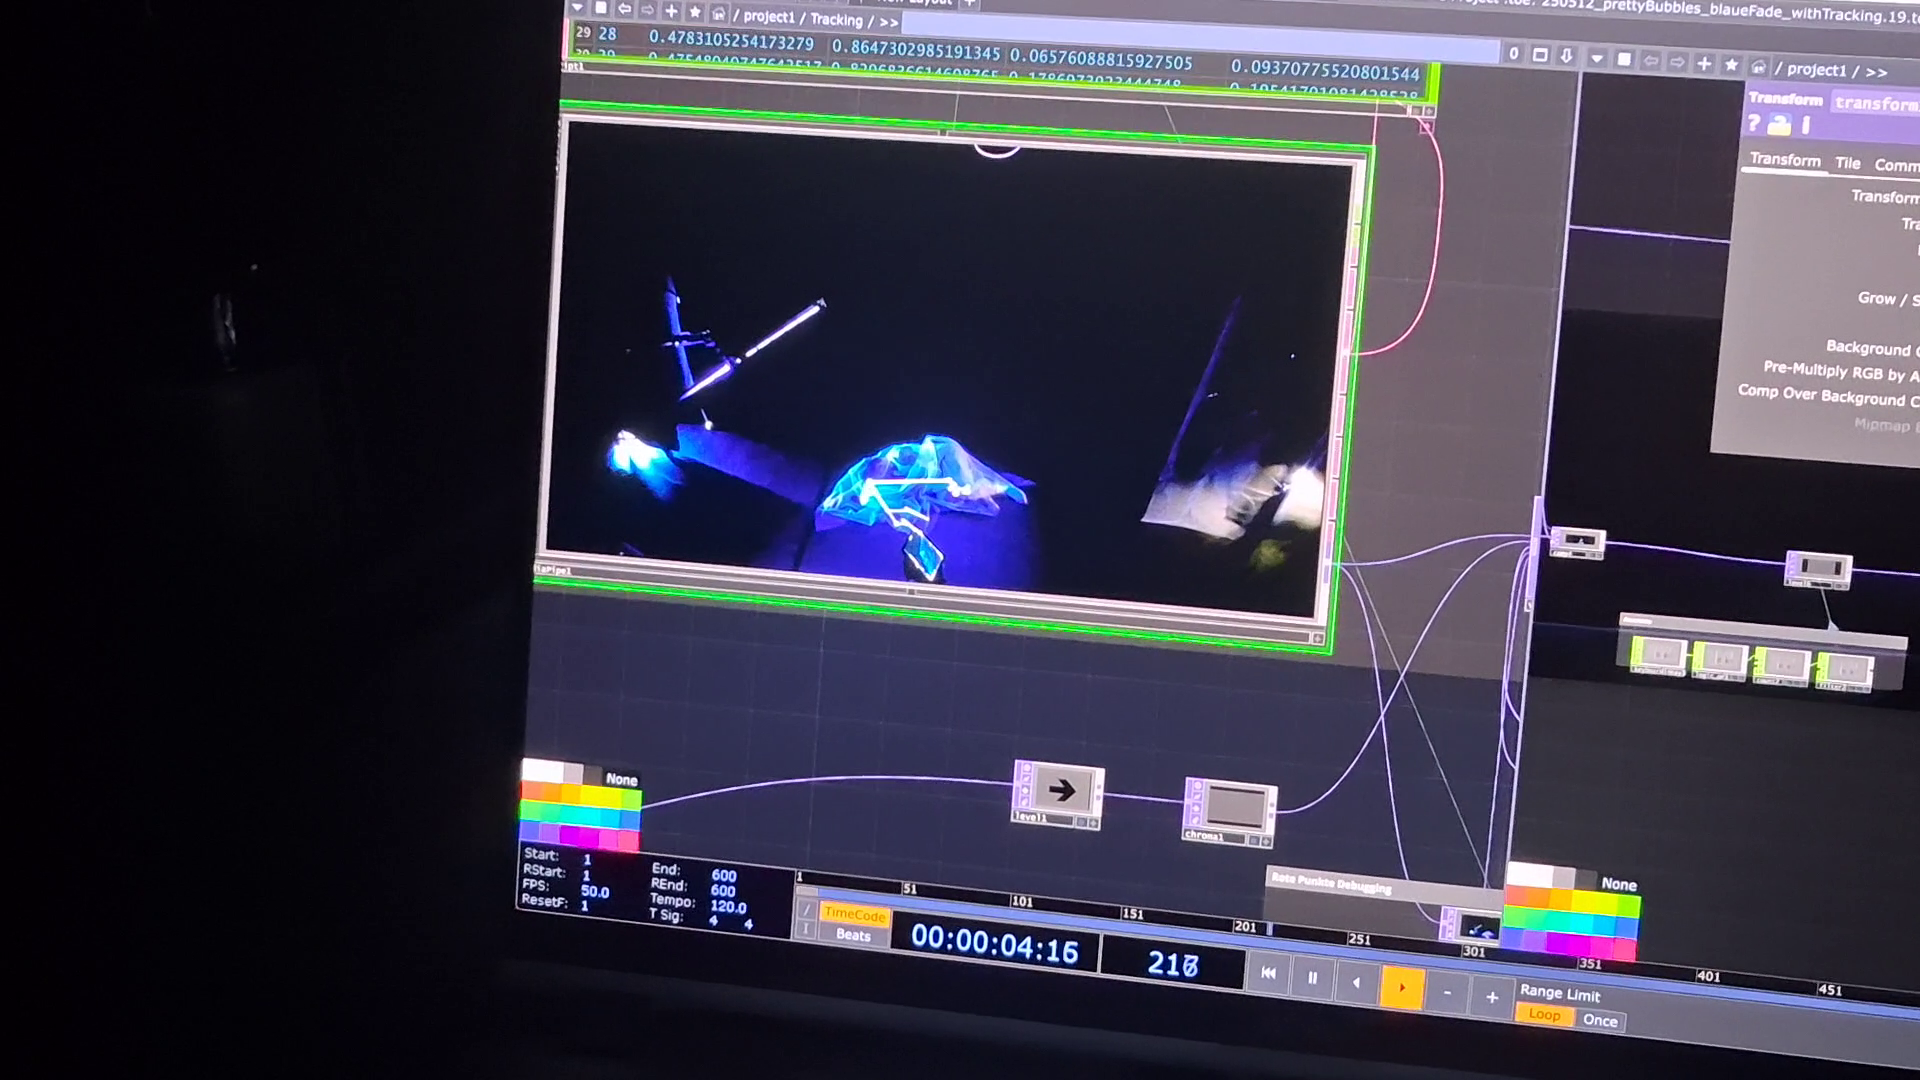
\includegraphics{images/onSetImages/DancerNotMediaPipeFoundCorrectlyWhenInClothOnFloor.png}%
    }
    \caption{Tracking-Problem: MediaPipe verliert Tänzer-Skelett-Erkennung bei Stoffverschleierung zu Beginn des Visuals -> Visuals werden manuell von mir anhand der Debug-Visualisierung an und dann zum Ende ausgeschaltet, wenn Ich sah, dass der Tänzer gut erkennt wird.}
    \label{fig:cloth_tracking_issue}
\end{figure}

\textbf{Professionelle Koordination:}

\raggedright Die Integration in professionelle Produktionsabläufe erforderte strukturierte Kommunikation technischer Anforderungen mit der Produktionsleitung. Diese Koordination zwischen technischen Systemanforderungen und kreativen Produktionszielen war ein wichtiger Aspekt des interdisziplinären Projektmanagements.

\textbf{Professionelle Entwicklung:}

\textbf{Vollständige Projektverantwortung:}

\raggedright Als einziger Entwickler trug ich die komplette technische Verantwortung. Jede Architekturentscheidung, jede Optimierung, jeder Workaround – alles lag in meiner Hand. Diese Erfahrung der vollständigen Ownership war gleichzeitig belastend und ermächtigend.

\textbf{Realistische Selbsteinschätzung:}

\raggedright Das Projekt lehrte mich, eigene Grenzen zu erkennen und zu kommunizieren. M.A.S.K. konkurriert nicht mit industriellen Motion-Capture-Systemen – und das ist in Ordnung. Diese Ehrlichkeit ermöglichte fokussierte Entwicklung statt feature creep.

\textbf{Nachhaltige Learnings:}

Drei Erkenntnisse prägen meine weitere Arbeit:

\textbf{1. Pragmatismus schlägt Perfektionismus:} Die funktionierende 80\%-Lösung ist wertvoller als die theoretische 100\%-Lösung.

\textbf{2. Interdisziplinarität erfordert Demut:} Andere Fachbereiche haben eigene Exzellenzkriterien, die respektiert werden müssen.

\textbf{3. Constraints fördern Kreativität:} \raggedright Die Limitierungen (Budget, Hardware, Zeit) zwangen zu alternativen Lösungen, die in einem ressourcenreichen Umfeld nie entstanden wären.

Die eigenständige Entwicklung von M.A.S.K. demonstriert, wie strukturierte Kommunikation und agile Methoden auch bei Solo-Projekten zu erfolgreicher interdisziplinärer Zusammenarbeit führen können.
